\documentclass{standalone}
\usepackage{tikz}
\usetikzlibrary{patterns, positioning}


\begin{document}
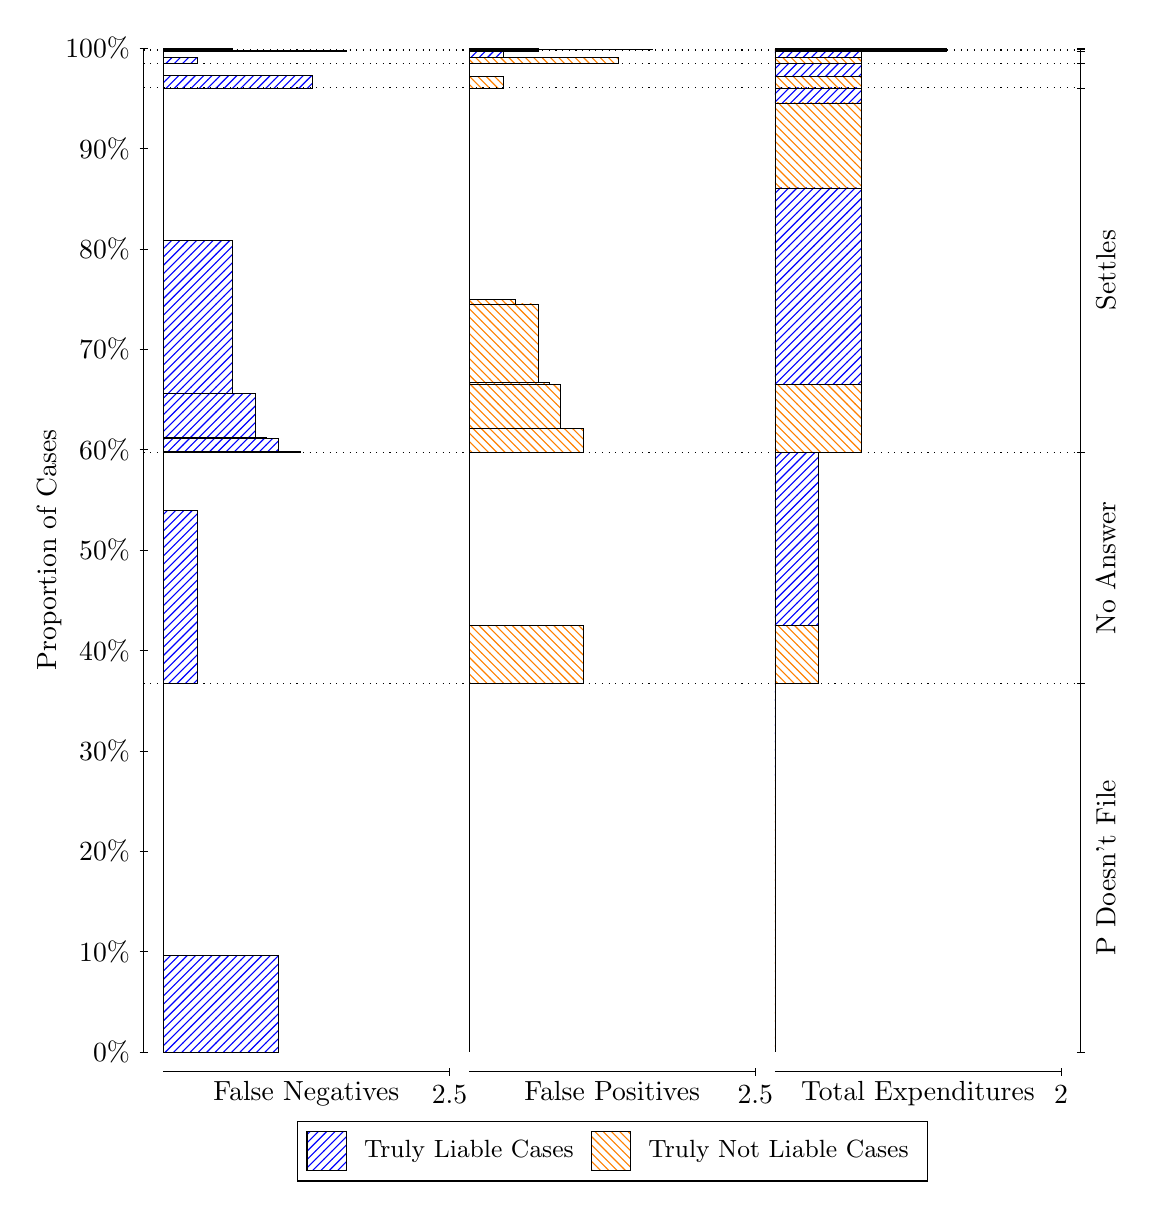
\begin{tikzpicture}
\draw[black, very thin] (1.5,1.75) -- (1.5,14.5);
\node[rotate=90, text=black, anchor=center] at (0.3, 8.125) {Proportion of Cases};
\draw[black, very thin] (1.45,1.75) -- (1.55,1.75);
\node[text=black, anchor=east] at (1.45, 1.75) {0\%};
\draw[black, very thin] (1.45,3.025) -- (1.55,3.025);
\node[text=black, anchor=east] at (1.45, 3.025) {10\%};
\draw[black, very thin] (1.45,4.3) -- (1.55,4.3);
\node[text=black, anchor=east] at (1.45, 4.3) {20\%};
\draw[black, very thin] (1.45,5.575) -- (1.55,5.575);
\node[text=black, anchor=east] at (1.45, 5.575) {30\%};
\draw[black, very thin] (1.45,6.85) -- (1.55,6.85);
\node[text=black, anchor=east] at (1.45, 6.85) {40\%};
\draw[black, very thin] (1.45,8.125) -- (1.55,8.125);
\node[text=black, anchor=east] at (1.45, 8.125) {50\%};
\draw[black, very thin] (1.45,9.4) -- (1.55,9.4);
\node[text=black, anchor=east] at (1.45, 9.4) {60\%};
\draw[black, very thin] (1.45,10.675) -- (1.55,10.675);
\node[text=black, anchor=east] at (1.45, 10.675) {70\%};
\draw[black, very thin] (1.45,11.95) -- (1.55,11.95);
\node[text=black, anchor=east] at (1.45, 11.95) {80\%};
\draw[black, very thin] (1.45,13.225) -- (1.55,13.225);
\node[text=black, anchor=east] at (1.45, 13.225) {90\%};
\draw[black, very thin] (1.45,14.5) -- (1.55,14.5);
\node[text=black, anchor=east] at (1.45, 14.5) {100\%};

\draw[black, very thin] (13.4,1.75) -- (13.4,14.5);
\draw[black, very thin] (13.35,1.75) -- (13.45,1.75);
\node[anchor=west] at (13.35, 1.75) {};
\draw[black, very thin] (13.35,6.4316) -- (13.45,6.4316);
\node[anchor=west] at (13.35, 6.4316) {};
\draw[black, very thin] (13.35,9.3657) -- (13.45,9.3657);
\node[anchor=west] at (13.35, 9.3657) {};
\draw[black, very thin] (13.35,13.995) -- (13.45,13.995);
\node[anchor=west] at (13.35, 13.995) {};
\draw[black, very thin] (13.35,14.302) -- (13.45,14.302);
\node[anchor=west] at (13.35, 14.302) {};
\draw[black, very thin] (13.35,14.464) -- (13.45,14.464);
\node[anchor=west] at (13.35, 14.464) {};
\draw[black, very thin] (13.35,14.48) -- (13.45,14.48);
\node[anchor=west] at (13.35, 14.48) {};
\draw[black, very thin] (13.35,14.5) -- (13.45,14.5);
\node[anchor=west] at (13.35, 14.5) {};

\draw[black, very thin, pattern color=blue, pattern=north east lines] (1.75,1.75) rectangle (3.2033,2.9803);
\draw[black, very thin, pattern color=orange, pattern=north west lines] (1.75,2.9803) rectangle (1.75,6.4316);
\draw[black, very thin, pattern color=blue, pattern=north east lines] (1.75,6.4316) rectangle (2.186,8.6274);
\draw[black, very thin, pattern color=orange, pattern=north west lines] (1.75,8.6274) rectangle (1.75,9.3657);
\draw[black, very thin, pattern color=blue, pattern=north east lines] (1.75,9.3657) rectangle (3.494,9.3806);
\draw[black, very thin, pattern color=blue, pattern=north east lines] (1.75,9.3806) rectangle (3.2033,9.5457);
\draw[black, very thin, pattern color=blue, pattern=north east lines] (1.75,9.5457) rectangle (3.058,9.5593);
\draw[black, very thin, pattern color=blue, pattern=north east lines] (1.75,9.5593) rectangle (2.9127,10.114);
\draw[black, very thin, pattern color=blue, pattern=north east lines] (1.75,10.114) rectangle (2.622,12.055);
\draw[black, very thin, pattern color=orange, pattern=north west lines] (1.75,12.055) rectangle (1.75,13.995);
\draw[black, very thin, pattern color=blue, pattern=north east lines] (1.75,13.995) rectangle (3.6393,14.155);
\draw[black, very thin, pattern color=orange, pattern=north west lines] (1.75,14.155) rectangle (1.75,14.302);
\draw[black, very thin, pattern color=blue, pattern=north east lines] (1.75,14.302) rectangle (2.186,14.382);
\draw[black, very thin, pattern color=orange, pattern=north west lines] (1.75,14.382) rectangle (1.75,14.464);
\draw[black, very thin, pattern color=blue, pattern=north east lines] (1.75,14.464) rectangle (4.0753,14.47);
\draw[black, very thin, pattern color=orange, pattern=north west lines] (1.75,14.47) rectangle (1.75,14.48);
\draw[black, very thin, pattern color=blue, pattern=north east lines] (1.75,14.48) rectangle (2.622,14.495);
\draw[black, very thin, pattern color=orange, pattern=north west lines] (1.75,14.495) rectangle (1.75,14.5);
\draw[black, very thin, pattern color=orange, pattern=north west lines] (5.6333,1.75) rectangle (5.6333,5.2013);
\draw[black, very thin, pattern color=blue, pattern=north east lines] (5.6333,5.2013) rectangle (5.6333,6.4316);
\draw[black, very thin, pattern color=orange, pattern=north west lines] (5.6333,6.4316) rectangle (7.0867,7.1699);
\draw[black, very thin, pattern color=blue, pattern=north east lines] (5.6333,7.1699) rectangle (5.6333,9.3657);
\draw[black, very thin, pattern color=orange, pattern=north west lines] (5.6333,9.3657) rectangle (7.0867,9.6725);
\draw[black, very thin, pattern color=orange, pattern=north west lines] (5.6333,9.6725) rectangle (6.796,10.229);
\draw[black, very thin, pattern color=orange, pattern=north west lines] (5.6333,10.229) rectangle (6.6507,10.256);
\draw[black, very thin, pattern color=orange, pattern=north west lines] (5.6333,10.256) rectangle (6.5053,11.251);
\draw[black, very thin, pattern color=orange, pattern=north west lines] (5.6333,11.251) rectangle (6.2147,11.306);
\draw[black, very thin, pattern color=blue, pattern=north east lines] (5.6333,11.306) rectangle (5.6333,13.995);
\draw[black, very thin, pattern color=orange, pattern=north west lines] (5.6333,13.995) rectangle (6.0693,14.143);
\draw[black, very thin, pattern color=blue, pattern=north east lines] (5.6333,14.143) rectangle (5.6333,14.302);
\draw[black, very thin, pattern color=orange, pattern=north west lines] (5.6333,14.302) rectangle (7.5227,14.384);
\draw[black, very thin, pattern color=blue, pattern=north east lines] (5.6333,14.384) rectangle (6.0693,14.464);
\draw[black, very thin, pattern color=orange, pattern=north west lines] (5.6333,14.464) rectangle (6.5053,14.474);
\draw[black, very thin, pattern color=blue, pattern=north east lines] (5.6333,14.474) rectangle (5.6333,14.48);
\draw[black, very thin, pattern color=orange, pattern=north west lines] (5.6333,14.48) rectangle (7.9587,14.485);
\draw[black, very thin, pattern color=blue, pattern=north east lines] (5.6333,14.485) rectangle (6.5053,14.5);
\draw[black, very thin, pattern color=orange, pattern=north west lines] (9.5167,1.75) rectangle (9.5167,5.2013);
\draw[black, very thin, pattern color=blue, pattern=north east lines] (9.5167,5.2013) rectangle (9.5167,6.4316);
\draw[black, very thin, pattern color=orange, pattern=north west lines] (9.5167,6.4316) rectangle (10.062,7.1699);
\draw[black, very thin, pattern color=blue, pattern=north east lines] (9.5167,7.1699) rectangle (10.062,9.3657);
\draw[black, very thin, pattern color=orange, pattern=north west lines] (9.5167,9.3657) rectangle (10.607,10.229);
\draw[black, very thin, pattern color=blue, pattern=north east lines] (9.5167,10.229) rectangle (10.607,12.724);
\draw[black, very thin, pattern color=orange, pattern=north west lines] (9.5167,12.724) rectangle (10.607,13.802);
\draw[black, very thin, pattern color=blue, pattern=north east lines] (9.5167,13.802) rectangle (10.607,13.995);
\draw[black, very thin, pattern color=orange, pattern=north west lines] (9.5167,13.995) rectangle (10.607,14.143);
\draw[black, very thin, pattern color=blue, pattern=north east lines] (9.5167,14.143) rectangle (10.607,14.302);
\draw[black, very thin, pattern color=orange, pattern=north west lines] (9.5167,14.302) rectangle (10.607,14.384);
\draw[black, very thin, pattern color=blue, pattern=north east lines] (9.5167,14.384) rectangle (10.607,14.464);
\draw[black, very thin, pattern color=orange, pattern=north west lines] (9.5167,14.464) rectangle (11.697,14.474);
\draw[black, very thin, pattern color=blue, pattern=north east lines] (9.5167,14.474) rectangle (11.697,14.48);
\draw[black, very thin, pattern color=orange, pattern=north west lines] (9.5167,14.48) rectangle (11.697,14.485);
\draw[black, very thin, pattern color=blue, pattern=north east lines] (9.5167,14.485) rectangle (11.697,14.5);
\draw[black, dotted] (1.5,6.4316) -- (13.4,6.4316);
\draw[black, dotted] (1.5,9.3657) -- (13.4,9.3657);
\draw[black, dotted] (1.5,13.995) -- (13.4,13.995);
\draw[black, dotted] (1.5,14.302) -- (13.4,14.302);
\draw[black, dotted] (1.5,14.464) -- (13.4,14.464);
\draw[black, dotted] (1.5,14.48) -- (13.4,14.48);
\draw[black, very thin] (1.75,1.5) -- (5.3833,1.5);
\node[text=black, anchor=north] at (3.5667, 1.5) {False Negatives};
\draw[black, very thin] (5.3833,1.45) -- (5.3833,1.55);
\node[text=black, anchor=north] at (5.3833, 1.45) {2.5};

\draw[black, very thin] (5.6333,1.5) -- (9.2667,1.5);
\node[text=black, anchor=north] at (7.45, 1.5) {False Positives};
\draw[black, very thin] (9.2667,1.45) -- (9.2667,1.55);
\node[text=black, anchor=north] at (9.2667, 1.45) {2.5};

\draw[black, very thin] (9.5167,1.5) -- (13.15,1.5);
\node[text=black, anchor=north] at (11.333, 1.5) {Total Expenditures};
\draw[black, very thin] (13.15,1.45) -- (13.15,1.55);
\node[text=black, anchor=north] at (13.15, 1.45) {2};

\node[text=black, centered, rotate=90] at (13.72, 4.0908) {P Doesn't File};
\node[text=black, centered, rotate=90] at (13.72, 7.8987) {No Answer};
\node[text=black, centered, rotate=90] at (13.72, 11.68) {Settles};





\draw (7.449999999999999,1.5) node[draw=none] (baseCoordinate) {};
\begin{scope}[align=center]
        \matrix[scale=0.5, draw=black, below=0.5cm of baseCoordinate, nodes={draw}, column sep=0.1cm]{
            \node[rectangle, draw, minimum width=0.5cm, minimum height=0.5cm, pattern color=blue, pattern=north east lines] {}; &
            \node[draw=none, font=\small, text=black] (B) {Truly Liable Cases}; &
            \node[rectangle, draw, minimum width=0.5cm, minimum height=0.5cm, pattern color=orange, pattern=north west lines] {}; &
            \node[draw=none, font=\small, text=black] (B) {Truly Not Liable Cases}; \\
            };
\end{scope}

\end{tikzpicture}
\end{document}